\documentclass{beamer}


%%%%%%%%% PACKAGES %%%%%%%%%%%%%%%%%
\usepackage[utf8]{inputenc}
\usepackage[T1]{fontenc}
\usepackage{amsmath}
\usepackage{amssymb}
\usepackage{amsfonts}
\usepackage{alltt}
\renewcommand{\ttdefault}{txtt} % to resolve a problem with bold fonts in alltt

\usepackage{listings}
\lstset{language=haskell,basicstyle=\ttfamily}

\usepackage{proof}
\inferLineSkip=4pt  % increase spacing between lines; default is 2pt

\usepackage[table]{xcolor}
\usepackage[colorlinks,hyperindex,bookmarks,linkcolor=blue,citecolor=blue,urlcolor=blue]{hyperref}
\usepackage{todonotes}

\usepackage{fancyhdr}

%\usepackage{floatflt}
\usepackage{wrapfig}
\usepackage{caption}
\usepackage{subcaption}
\usepackage{framed}
\usepackage{multicol}

\makeatletter

\usepackage{babel}
\usepackage{graphicx}
\usepackage{theorem}

\usepackage{tikz}
\usetikzlibrary{trees}
\usetikzlibrary{positioning} 
\usepackage{tikzsymbols}


\makeatother

%%%%%%%%% GEOMETRY %%%%%%%%%%%%%%%%%
\addtolength{\topmargin}{-15mm}
\addtolength{\textheight}{25mm}
\addtolength{\oddsidemargin}{-20mm}
\setlength{\textwidth}{16cm}

%%%%%%%%% DECLS / DEFNS %%%%%%%%%%%%%%%%%

\usepackage{comment}
\specialcomment{solution}
{\todo[inline]{BEGIN SOLUTION}}
{\todo[inline]{END SOLUTION}}

{\theorembodyfont{\rmfamily} 
  \newtheorem{exo}{Exercise}
  \newtheorem{rem}{Remark}
}

% Macros for references
\newcommand{\polyref}[1]{polycopié, {#1}}

%%%%%%%%% END DECLS / DEFNS %%%%%%%%%%%%%%%%%

%%% Local Variables: 
%%% mode: latex
%%% coding: utf-8-unix
%%% End: 

% Theorems and definitions

% \newtheorem{definition}{Definition}
% \newtheorem{theorem}{Theorem}
% \newtheorem{lemma}{Lemma}
% \newtheorem{proposition}{Proposition}


% Definition of colors
\newcommand{\blue}[1]{{\color{blue}#1}}
\newcommand{\green}[1]{{\color{green}#1}}
\newcommand{\red}[1]{{\color{red}#1}}
\newcommand{\gray}[1]{{\color{gray}#1}}

% From MSCS file
\newcommand{\eg}{\textit{e.g.\ }}
\newcommand{\etal}{\textit{et al.\ }}
\newcommand{\etc}{\textit{etc}}
\newcommand{\ie}{\textit{i.e.\ }}
\newcommand{\viz}{\textit{viz.\ }}
\newcommand{\wrt}{\textit{w.r.t.\ }}
\newcommand{\lex}{\langle}
\newcommand{\rex}{\rangle}

% Own abbreviations
\newcommand{\secref}[1]{Section~\ref{#1}}
\newcommand{\secrefs}[1]{Sections~\ref{#1}}
\newcommand{\figref}[1]{Figure~\ref{#1}}
\newcommand{\figrefs}[1]{Figures~\ref{#1}}
\newcommand{\pgref}[1]{page~\pageref{#1}}
\newcommand{\theoremref}[1]{Theorem~\ref{#1}}
\newcommand{\theoremrefs}[1]{Theorems~\ref{#1}}
\newcommand{\lemmaref}[1]{Lemma~\ref{#1}}
\newcommand{\exampleref}[1]{Example~\ref{#1}}
\newcommand{\defref}[1]{Definition~\ref{#1}}

\newcommand{\figline}{\rule{\textwidth}{0.5pt}}


% Logique

\newcommand{\IMPL}[0]{\longrightarrow}
\newcommand{\IMPLL}[0]{\Longrightarrow} % another implication, to make
                                % a difference with reduction relations
\newcommand{\AND}[0]{\land}
\newcommand{\OR}[0]{\lor}
\newcommand{\NOT}[0]{\lnot}
\newcommand{\FALSE}[0]{\perp}
\newcommand{\TRUE}[0]{\top}
\newcommand{\IFF}[0]{\leftrightarrow}
\newcommand{\BIGAND}[1]{\bigwedge_{#1}}
\newcommand{\BIGOR}[1]{\bigvee_{#1}}
\newcommand{\BIGANDC}[2]{\bigwedge_{#1|#2}} % bigand with constraint
\newcommand{\BIGORC}[2]{\bigvee_{#1|#2}}    % bigor with constraint

\newcommand{\exgeq}[1]{\exists^{{\geq #1}}}
\newcommand{\exeq}[1]{\exists^{{= #1}}}
\newcommand{\exle}[1]{\exists^{{< #1}}}

% Remark macros for the authors

\newcommand{\remms}[2][]{\todo[color=green!40,#1]{MS: #2}}
\newcommand{\remre}[2][]{\todo[color=blue!40,#1]{RE: #2}}
\newcommand{\remjhb}[2][]{\todo[color=blue!20,#1]{JHB: #2}}


% Other

\newcommand{\smalltalcq}[0]{{\small small}-t{$\cal ALCQ$}}
\newcommand{\smalltalcqe}[0]{{\small small}-t{$\cal ALCQ$e}}
\newcommand{\trule}[0]{\xhookrightarrow}
\newcommand{\tableaurule}[1]{{\xhookrightarrow[]{#1}}}
\newcommand{\nodes}[1]{{\cal N}({#1})}
\newcommand{\trans}[1]{{\cal T}({#1})}
\newcommand{\transm}[1]{{\cal T'}({#1})}
\newcommand{\rconts}[1]{\llparenthesis #1 \rrparenthesis} %record contents
\newcommand{\rupd}[2]{{#1}\llparenthesis #2 \rrparenthesis} %record update

\newcommand{\eform}[0]{\mathit{eform}}
\newcommand{\form}[0]{\mathit{form}}
\newcommand{\free}[0]{\mathit{free}}
\newcommand{\exclprop}[0]{\stackrel{\times}{\longrightarrow}}

%%% Local Variables: 
%%% mode: latex
%%% TeX-master: "main"
%%% End: 


\title{Propositional and Predicate Logic}

\author{Martin Strecker}
\date{2020-11-20}


%======================================================================

\begin{document}


%======================================================================

\begin{frame}
  \titlepage
\end{frame}



%======================================================================
\section{Propositional Logic}

%-------------------------------------------------------------
\subsection{Syntax}
%-------------------------------------------------------------

%-------------------------------------------------------------
\begin{frame}[fragile]\frametitle{Recap: Propositional logic -- Syntax}


  \begin{columns}[t]
    \column{.5\textwidth}
    \blue{As grammar (\emph{concrete} syntax)}

    \vspace{3mm}
  \begin{tabular}{rcl}
    Form  & ::=  & $\TRUE$ \\
          & | &  $\FALSE$ \\
          & | &  Var\\
          & | &  $\NOT$ Form \\
          & | &  Form $\AND$ Form \\
          & | &  Form $\OR$ Form \\
  \end{tabular}

    \column{.5\textwidth}
  \blue{In Haskell (\emph{abstract} syntax):}
\begin{lstlisting}
data Form
  = C Bool
  | V String
  | Not Form
  | Form `And` Form
  | Form `Or` Form
\end{lstlisting}
\end{columns}  

\end{frame}

%-------------------------------------------------------------
\begin{frame}[fragile]\frametitle{Concrete vs. abstract syntax}

  \blue{Concrete syntax:} the way you write down a formula, often with:
  \begin{itemize}
  \item explicit parentheses
  \item implicit rules of precedence: \\
    \emph{in decreasing strength:} $\NOT >  \AND > \OR > \IMPL$\\
    \emph{Ex:}  $\NOT p \AND q \IMPL p \OR r$ $\leadsto$ $((\NOT p) \AND q) \IMPL (p \OR r)$
  \item implicit rules of associativity: \\
    $\IMPL$ associates to the left:\\
    \emph{Ex.:} $A \IMPL B \IMPL C$ $\leadsto$ $A \IMPL (B \IMPL C)$
  \end{itemize}

\end{frame}

%-------------------------------------------------------------
\begin{frame}[fragile]\frametitle{Concrete vs. abstract syntax}

  \blue{Abstract syntax:} Corresponding to the internal representation

  \emph{Ex.:} concrete syntax: $(p \OR q) \AND (s \AND \NOT r) \OR \NOT s$

  \vspace{5mm}
  In Haskell (fully parenthesized!):
  \begin{lstlisting}
 ((((V p) `Or` (V q)) `And` ((V s) `And` (Not (V r)))) 
    `Or` (Not (V s)))
  \end{lstlisting}
  

  \vspace{5mm}
  As syntax tree:
\begin{center}
\mbox{
\xymatrix@=1mm{ &        &       &       &    & \OR\ar@{-}[llld]\ar@{-}[rd] &      &    \\
           &    & \AND\ar@{-}[ld]\ar@{-}[rrd]  &       &    &       & \NOT\ar@{-}[d] &    \\
          &  \OR\ar@{-}[ld]\ar@{-}[rd]  &   &    & \AND\ar@{-}[ld]\ar@{-}[rd]   &       &   s &   \\
        p   &        & q &  s         &   & \NOT\ar@{-}[d]       &      &    \\
          &        &  &           &   & r       &      &    
  }}
\end{center}
\end{frame}


%-------------------------------------------------------------
\subsection{Semantics}
%-------------------------------------------------------------


%-------------------------------------------------------------
\begin{frame}[fragile]\frametitle{Recap: Propositional logic -- Semantics}


  \blue{Valuation:} Assignment of truth values (0 / 1) to propositional variables.

  Computing the truth value of a complex formula from its constituents:
  
  \blue{Truth table}
  \begin{center}
  \begin{tabular}{|c|c||c|c|c|c|}
    \hline
    $A$ & $B$ &  $\NOT A$ & $A \AND B$ & $A \OR B$ \\
    \hline
    0   & 0   &  1 & 0          & 0	\\
    0   & 1   &  1 & 0          & 1    \\
    1   & 0   &  0 & 0          & 1	\\
    1   & 1   &  0 & 1          & 1	\\
    \hline
  \end{tabular}
  \end{center}

\end{frame}


%-------------------------------------------------------------
\begin{frame}[fragile]\frametitle{Truth tables}

\blue{Truth table of  $(p \AND q) \OR (\NOT r)$}
  \begin{center}
  \begin{tabular}{c|c|c||c|c||cl}
    \hline
    $p$ & $q$ & $r$ & $p \AND q$ & $\NOT r$ & $(p \AND q) \OR (\NOT r)$ & \\  \hline \hline
    0   & 0   & 0   & 0          & 1        & 1                         & \\ \hline
    0   & 0   & 1   & 0          & 0        & 0                         & \\ \hline
    0   & 1   & 0   & 0          & 1        & 1                         & \\ \hline
    0   & 1   & 1   & 0          & 0        & 0                         & \\ \hline
    \red{1} & \red{0}   & \red{0}   & \red{0}   & \red{1}  & \red{1}    & $\leftarrow$ model\\ \hline
    1   & 0   & 1   & 0          & 0        & 0                         & \\ \hline
    1   & 1   & 0   & 1          & 1        & 1                         & \\ \hline
    1   & 1   & 1   & 1          & 0        & 1                         & \\ \hline
  \end{tabular}
  \end{center}

  Each line corresponds to a \emph{valuation}.
  \begin{itemize}
  \item \emph{valid:} all lines 1
  \item \emph{unsatisfiable:} all lines 0
  \item \emph{contingent:} otherwise
  \end{itemize}

\end{frame}

%-------------------------------------------------------------
\begin{frame}[fragile]\frametitle{Implication}

  You are cashier in a restaurant and have to enforce the rule:

  \begin{center}
    \red{alcohol $\IMPL$ major}
  \end{center}

    \begin{columns}[t]
    \column{.6\textwidth}
  \begin{tabular}{|c|c||c|}
    \hline
    drink & age & alcohol $\IMPL$ major	\\  \hline \hline
    coffee   &  13   & \pause \Smiley			\\ \hline
    coffee   &  21   & \pause \Smiley			\\ \hline
    beer     &  13   & \pause \Sadey			\\ \hline
    beer     &  21   & \pause \Smiley			\\ \hline
  \end{tabular}
  \column{.3\textwidth}
  \pause
  \begin{tabular}{|c|c||c|}
    \hline
    A & M & A $\IMPL$ M	\\  \hline \hline
    0   &  0   & 	1		\\ \hline
    0   &  1   & 	1		\\ \hline
    1   &  0   & 	0		\\ \hline
    1   &  1   & 	1		\\ \hline
  \end{tabular}

  \vspace{3mm}
  $A \IMPL M \equiv \NOT A \OR M$
\end{columns}

\end{frame}

%-------------------------------------------------------------
\begin{frame}[fragile]\frametitle{Validity and Counter-models}

  \emph{Example:} ``Socrates is a human. Every human is mortal. Thus, Socrates is mortal'':

  \vspace{3mm}
  Let $f_1$ be: $h \AND (h \IMPL m) \IMPL m$

  \begin{itemize}
  \item $f_1$ is \emph{valid} (true for all valuations)\\
    brute force: compute all valuations.
  \end{itemize}


  \vspace{3mm}
  Take instead $f_2$ to be: $h \AND (m \IMPL h) \IMPL m$

  \begin{itemize}
  \item $f_2$ is \emph{satisfiable} (interpret $m \mapsto 1$)
  \item but \emph{not valid}: 
    interpretation $h \mapsto 1, m \mapsto 0$ is a \emph{counter-model}
    refuting $f_2$
  \end{itemize}
  
  
\end{frame}


%======================================================================
\section{Predicate Logic}


%-------------------------------------------------------------
\subsection{Syntax}
%-------------------------------------------------------------

%-------------------------------------------------------------
\begin{frame}[fragile]\frametitle{Shortcomings of Propositional Logic}

  \emph{Example:} ``Socrates is a human. Every human is mortal. Thus, Socrates is mortal'':

  $h \AND (h \IMPL m) \IMPL m$

  \vspace{3mm}

  \emph{Question}: How to model: \\
  ``Plato is a human. Every human is mortal. Thus, Plato is mortal''

  \vspace{3mm}
  Suggestions:
  \begin{enumerate}
  \item $h \AND (h \IMPL m) \IMPL m$\\
    Difference to the above?
  \item $hs \AND (hs \IMPL ms) \IMPL ms$ and\\
    $hp \AND (hp \IMPL mp) \IMPL mp$\\
    Redundant!
  \item $hs \AND hp \AND (h \IMPL m) \IMPL ms \AND mp$\\
    Relation between $hs / hp$ and $h$?
  \end{enumerate}

\end{frame}

%-------------------------------------------------------------
\begin{frame}[fragile]\frametitle{Towards Predicate Logic}

  \blue{Predicate Logic} is an \emph{extension} of Propositional Logic:
  \begin{itemize}
  \item Keep logical constants $\TRUE, \FALSE$ and connectors $\NOT, \AND, \OR$
  \item Instead of \emph{propositional variables}, introduce \emph{predicates}:\\
    $hs, hp$ $\leadsto$ $Human(socrates), Human(plato)$
  \item Introduce \emph{quantifiers:}
    \begin{itemize}
    \item universal (``for all''): $\forall x. P(x)$
    \item existential (``for some / exists''): $\exists x. P(x)$
    \end{itemize}
  \end{itemize}

  Now easy to express:

  \begin{itemize}
  \item $Human(socrates) \AND Human(plato)$
  \item $\forall x.\; Human(x) \IMPL Mortal(x)$
  \item $Mortal(socrates) \AND Mortal(plato)$
  \end{itemize}

\end{frame}

%-------------------------------------------------------------
\begin{frame}[fragile]\frametitle{Syntax of Predicate Logic}

  \begin{tabular}{rcl}
    Form  & ::=  & $\TRUE$ \\
          & | &  $\FALSE$ \\
          & | &  \red{$P(Term, \dots Term)$}\\
          & | &  $\NOT$ Form \\
          & | &  Form $\AND$ Form \\
          & | &  Form $\OR$ Form \\
          & | &  \red{$\forall x. Form$}\\
          & | &  \red{$\exists x. Form$}\\
  \end{tabular}

  Questions:
  \begin{enumerate}
  \item In Haskell?\\
    Dealing with \emph{bound variables} not so easy, see below.
  \item What is a $Term$?
  \end{enumerate}
  
\end{frame}

%-------------------------------------------------------------
\begin{frame}[fragile]\frametitle{Predicates and Functions}

A \blue{predicate} makes a statement about facts involving one or several
objects. The objects are the \emph{arguments}:
\begin{itemize}
\item $Human(plato)$
\item $Loves(john, mary)$
\item $Less(2, 3)$ often written infix: $2 < 3$
\end{itemize}


A \blue{function} describes a transformation of an object (and produces a new
object):
\begin{itemize}
\item $boil(egg, 3min)$
\item $paint(paint(table, red), blue)$
\item $plus(2, times(3, 4))$ sometimes written infix: $2 + (3 * 4)$
\end{itemize}

\end{frame}

%-------------------------------------------------------------
\begin{frame}[fragile]\frametitle{Predicates and Functions}

  A \blue{term} represents an object in the domain of discourse. It can be:
  \begin{itemize}
  \item a constant: $3, 42$, $john$, $mary$
  \item a variable: $x, y, \dots$
  \item a function applied to terms: $2 + 3$, $paint(table, red)$
  \end{itemize}

  \vspace{3mm}
  A \emph{constant} can be understood as a function with no arguments:\\ $2$ the same as $2()$.

  \vspace{3mm}

  \begin{tabular}{rcl}
    Term  & ::=  & $IVar$ \\
          & | &  $Fun(Term, \dots, Term)$
  \end{tabular}
  
  where:
  \begin{itemize}
  \item $IVar$: set of \emph{individual variables} (contrary to
    \emph{propositional variables})
  \item $Fun$: set of function symbols
  \end{itemize}

\end{frame}

%-------------------------------------------------------------
\begin{frame}[fragile]\frametitle{What you may and may not write}

  \red{Attention:} the arguments of a predicate are terms and not formulas

  \emph{Ex.:} ``Eve eats an apple that she has bought'':
  \begin{itemize}
  \item \red{False:} $Eats(eve, Buy(eve, apple))$
  \item \green{Correct:} $Buy(eve, apple) \IMPL Eats(eve, apple)$
  \end{itemize}

  \vspace{3mm}
  By convention:
  \begin{itemize}
  \item in classical logic: funs, vars: lower case; predicates: upper case
  \item in Prolog: predicates, functions: lower case; vars: upper case
  \end{itemize}

\end{frame}

%-------------------------------------------------------------
\begin{frame}[fragile]\frametitle{Limits of expressivity}

  \blue{Temporal properties} not directly expressible:
  \begin{itemize}
  \item ``One will eventually pay for every item one has bought''
  \item but can be coded: $\forall b, i, t.\; Buy(b, i, t) \IMPL (\exists t'. t'
    > t \AND Pay(b, i, t'))$
  \end{itemize}

  \vspace{5mm}
  \blue{Modal} or \blue{deontic statements} not directly expressible:
  \begin{itemize}
  \item ``It is \emph{necessary} to pay for every item bought''
  \item ``It is \emph{obligatory} to pay for every item bought''
  \item but codings possible
  \end{itemize}
  
\end{frame}

%-------------------------------------------------------------
\begin{frame}[fragile]\frametitle{Limits of expressivity}

  \blue{First-order logic} only quantifies about objects
  \begin{itemize}
  \item but not about functions: ``Every function has an inverse'':\\
    \red{Forbidden:} $\forall f. \exists g. \forall x. f(g(x)) = x$\\
    (higher-order quantification)
  \item and not about predicates: ``Love is always reciprocal'':\\
    \red{Forbidden:} $Sym(Love)$ where $Sym(R) = \forall x, y. R(x, y) \IFF
    R(y, x)$
    (higher-order functions / predicates)
  \end{itemize}
  Higher-order features \emph{not} codable in first-order logic.
  
\end{frame}

%-------------------------------------------------------------
\begin{frame}[fragile]\frametitle{Some hairy details about bound variables}

  ``Every human is mortal'': consider the following as identical:
  \begin{itemize}
  \item $\forall x. Human(x) \IMPL Mortal(x)$
  \item $\forall p. Human(p) \IMPL Mortal(p)$
  \end{itemize}

  Renaming of bound variables, just as in:
  \begin{lstlisting}
    map (\x -> x + 2) [1, 2, 3]
    map (\n -> n + 2) [1, 2, 3]
  \end{lstlisting}

  Can we rename arbitrarily? Certainly not!\\
  Compare: ``Everybody is loved by somebody''
  \begin{itemize}
  \item $\forall x. \exists y. Loves(x, y)$
  \item $\forall x. \exists x. Loves(x, x)$
  \end{itemize}

\end{frame}



%-------------------------------------------------------------
\subsection{Semantics}
%-------------------------------------------------------------

%-------------------------------------------------------------
\begin{frame}[fragile]\frametitle{Interpretations}

  \blue{Formally:} Extend the notion of \emph{valuation} to an
  \emph{interpretation}.\\
  Very technical!

  \vspace{5mm}
  \blue{Informally:}
  \begin{itemize}
  \item \emph{Unary predicates} can be understood as representing \emph{sets}:\\
    \emph{Ex.:} $SGCitizen(x)$ the set of Singapore citizens\\
    $\forall x. SGCitizen(x) \IMPL AsianCitizen(x)$: the set of SG citizens is
    a subset of Asian citizens.
  \end{itemize}

\end{frame}


%-------------------------------------------------------------
\begin{frame}[fragile]\frametitle{Interpretation}
  \begin{itemize}
  \item \emph{Binary predicates:} represent relations/ arcs in a graph.\\
    \emph{Ex.:}
    \begin{itemize}
    \item $res(p,r)$: person $p$ has residence $r$
    \item $parents(c, p)$: child $c$ has parent $p$
    \end{itemize}
  \end{itemize}

\begin{center}
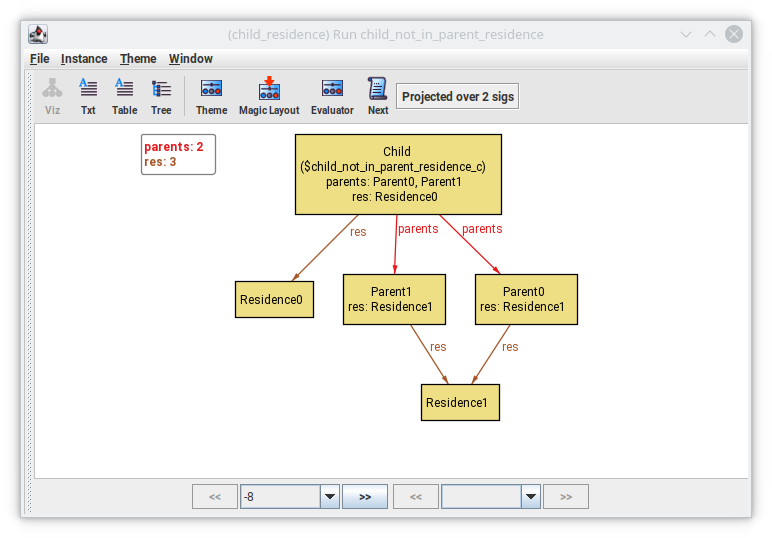
\includegraphics[width=0.7\textwidth]{child_residence_alloy_model.png}
\end{center}
  
\end{frame}

%-------------------------------------------------------------
\begin{frame}[fragile]\frametitle{Quantification over finite and infinite domains}


  \begin{itemize}
  \item ``All elements in $\{1, 2, 3\}$ are even'' (a false statement):\\
    $\forall x \in \{1, 2, 3\}. even(x)$
  \item ``There is an even element in $\{1, 2, 3\}$'' (correct):\\
    $\exists x \in \{1, 2, 3\}. even(x)$
  \end{itemize}

  In Haskell:
  \begin{lstlisting}
    all (\x -> even x) [1, 2, 3]
    any (\x -> even x) [1, 2, 3]
  \end{lstlisting}

  Knowing that \texttt{($\backslash$x -> even x)} is pointwise equal to \texttt{even}:
  \begin{lstlisting}
    all even [1, 2, 3]
    any even [1, 2, 3]
  \end{lstlisting}

\end{frame}

%-------------------------------------------------------------
\begin{frame}[fragile]\frametitle{Quantification over finite and infinite domains}

  Definition of \texttt{all / any} in Haskell, see\\
  \url{https://www.haskell.org/onlinereport/haskell2010/haskellch9.html}

  \begin{lstlisting}
and, or          :: [Bool] -> Bool  
and              =  foldr (&&) True  
or               =  foldr (||) False

any, all         :: (a -> Bool) -> [a] -> Bool  
any p            =  or . map p  
all p            =  and . map p 
  \end{lstlisting}
  
\end{frame}

%-------------------------------------------------------------
\begin{frame}[fragile]\frametitle{Quantification over finite and infinite domains}

  Let's unfold the \texttt{foldr}:

  \begin{itemize}
  \item \texttt{all even [1, 2, 3]}\\
    $\leadsto$ \texttt{(even 1) \&\& (even 2) \&\& (even 3) \&\& True}
  \item \texttt{any even [1, 2, 3]}\\
    $\leadsto$ \texttt{(even 1) || (even 2) || (even 3) || False}
  \end{itemize}

  Thus:
  \begin{itemize}
  \item Universal quantification $\forall$ (over a finite domain / unrestricted) can be
    assimilated to (finite / infinite) conjunction $\AND$
  \item Existential quantification $\exists$ (over a finite domain / unrestricted) can be
    assimilated to (finite / infinite) disjunction $\OR$
  \end{itemize}

\end{frame}

%-------------------------------------------------------------
\begin{frame}[fragile]\frametitle{Understanding Properties of Quantification}

  \blue{Duality:}
  \begin{itemize}
  \item of conjunction / disjunction:\\
    $\NOT (A \AND B) \equiv (\NOT A) \OR (\NOT B)$ and
    $\NOT (A \OR B) \equiv (\NOT A) \AND (\NOT B)$

  \item of quantifiers, assuming $x$ ranges over domain $\{d_1, d_2, \dots \}$:\\
    $\NOT (\forall x. P(x)) \equiv \NOT (P(d_1) \AND P(d_2) \AND \dots)$\\
    $\equiv (\NOT P(d_1) \OR \NOT P(d_2) \OR \dots)$
    $\equiv \exists x. \NOT P(x)$
  \item similarly: $\NOT (\exists x. P(x)) \equiv \forall x. \NOT P(x)$

  \end{itemize}

\end{frame}

%-------------------------------------------------------------
\begin{frame}[fragile]\frametitle{Understanding Properties of Quantification}


  \blue{Exchange} of quantifiers: 
  \begin{itemize}
  \item $\forall x. \forall y. R(x,y)$\\
    $\equiv (R(d_1,d_1) \AND R(d_1,d_2) \dots) \AND (R(d_2,d_1) \AND R(d_2,d_2)) \dots$\\
    $\equiv (R(d_1,d_1) \AND R(d_2,d_1) \dots) \AND (R(d_1,d_2) \AND  R(d_2,d_2)) \dots$\\
    $\equiv \forall y. \forall x. R(x,y)$
  \item similarly: $\exists x. \exists y. R(x,y) \equiv \exists y. \exists x. R(x, y)$
  \end{itemize}


  \vspace{5mm}
  \blue{Distributivity} of quantifiers over connectors:
  \begin{itemize}
  \item $\forall x. (P(x) \AND Q(x)) \equiv (\forall x. P(x)) \AND (\forall x. Q(x))$ 
  \item $\exists x. (P(x) \OR Q(x)) \equiv (\exists x. P(x)) \OR (\exists x. Q(x))$ 
  \end{itemize}

\end{frame}

%-------------------------------------------------------------
\begin{frame}[fragile]\frametitle{Counter-models}


  Does the following equality hold?\\
  $\forall x. \exists y. R(x,y) \equiv \exists y. \forall x. R(x,y)$


  \pause
  \vspace{3mm}
  \red{No!} Construct a \emph{counter-model} 
  \begin{itemize}
  \item extends the notion of counter-model of propositional logic.
  \item \emph{here:} take domain of interpretation to be $\mathbb{N}$ and $R$
    the relation $<$. Then:
    \begin{itemize}
    \item $\forall x. \exists y. x < y$ holds\\
      (take, for example, $y = x + 1$)
    \item $\exists y. \forall x. x < y$ does not hold\\
      (there is no $y$ bigger than all numbers)
    \end{itemize}
  \end{itemize}

  \vspace{3mm}
  In a similar spirit, refute:\\
  $\forall x. P(x) \OR Q(x) \equiv (\forall x. P(x)) \OR (\forall x. Q(x))$
\end{frame}



\end{document}


%%% Local Variables: 
%%% mode: latex
%%% TeX-master: t
%%% coding: utf-8
%%% End: 
